\documentclass[journal,10pt,twocolumn]{article}
\usepackage{graphicx, float}
\usepackage[margin=0.5in]{geometry}
\usepackage{amsmath, bm}
\usepackage{array}
\usepackage{booktabs}
\providecommand{\norm}[1]{\lVert#1\rVert}
\let\vec\mathbf
\newcommand{\myvec}[1]{\ensuremath{\begin{pmatrix}#1\end{pmatrix}}}
\newcommand{\mydet}[1]{\ensuremath{\begin{vmatrix}#1\end{vmatrix}}}

\title{\textbf{CONIC}}
\author{VEMULAPALLI BAVYA SRI}
\date{October 2022}

\begin{document}

\maketitle
\paragraph{\textit{Problem Statement} - A tangent to the ellipse $x^2 + 4y^2 = 4$ meets the ellipse $x^2 + 2y^2 = 6$ at P and Q. Prove that the tangents at P and Q of the ellipse $x^2 + 2y^2 = 6$ are at right angles.}
  
\section{Solution}

    Given, 
    
    \begin{equation}
    \label{eqn:1}
        \vec{x^2} + 4\vec{y^2} =  4
    \end{equation}
    
    \begin{flushleft}
        The standard equation of the conics is given as
    \end{flushleft}
    
    \begin{equation}
    \label{eqn:2}
        \Vec{x^\top}\Vec{V}\Vec{x} + 2\Vec{u^\top}\Vec{x} + f = 0
    \end{equation}
    
    \begin{flushleft}
        By Comparing \eqref{eqn:1} and \eqref{eqn:2} we get,
    \end{flushleft}
    
    \begin{equation}
    \label{eqn:3}
        \Vec{V_1} = \myvec{1 & 0 \\ 0 & 4} , \Vec{u_1} = \myvec{0 \\ 0} , f_1 = -4
    \end{equation}

    \begin{flushleft}
        Equation of the ellipse is given as,
    \end{flushleft}
    
    \begin{equation}
    \label{eqn:4}
        \vec{x^2} + 2\vec{y^2} = 6
    \end{equation}

    \begin{flushleft}
        By comparing \eqref{eqn:4} with \eqref{eqn:2}, we get
    \end{flushleft}
    
    \begin{equation}
    \label{eqn:5}
        \Vec{V_2} = \myvec{1 & 0 \\ 0 & 2} , \Vec{u_2} = \myvec{0 \\ 0} , f_2 = -6
    \end{equation}
    
    \begin{flushleft}
        On substituting these values in the standard equation of conics, we get
    \end{flushleft}
    
    \begin{equation}
    \label{eqn:6}
        \vec{x^\top}\myvec{1 & 0 \\ 0 & 2}\vec{x} - 6 = 0 
    \end{equation}
    
    \begin{flushleft}
        If $\vec{q}$ is the point of contact of the tangent to the ellipse then standard equation of the tangent to the conic is given as
    \end{flushleft}
    
    \begin{equation}
    \label{eqn:7}
        (\Vec{Vq + u})^\top\vec{x} + \vec{u}^\top\vec{q} + f = 0
    \end{equation}

    \subsection{Equation of tangent at $\vec{q_1}$}
    \begin{equation}
    \label{eqn:8}
        Let \ \vec{q_1} = \myvec{0 \\ 1}
    \end{equation}
    
    \begin{flushleft}
        By substituting \eqref{eqn:8} and \eqref{eqn:3} in \eqref{eqn:7} we get the equation of tangent as
    \end{flushleft}
    
    \begin{equation}
    \label{eqn:9}
        \myvec{0 & 4}\vec{x} = 4
    \end{equation}
    
    \begin{flushleft}
        By comparing \eqref{eqn:9} with the standard vector equation, we get 
    \end{flushleft}
    
    \begin{equation}
    \label{eqn:10}
        \Vec{n} = \myvec{0 \\ 4} , \vec{m} = \myvec{-4 \\ 0}
    \end{equation}
    
    \begin{flushleft}
        Points of intersection of the line (\eqref{eqn:9}) with the curve (\eqref{eqn:6}) are given by
    \end{flushleft}
    
    \begin{equation}
    \label{eqn:11}
        \vec{x}_i = \vec{q_1} + \mu_i\vec{m}
    \end{equation}
    
    \begin{flushleft}
        On solving we get the points of intersection as
    \end{flushleft}
    
    \begin{equation}
    \label{eqn:12}
        \vec{P} = \myvec{-2 \\ 1} , \vec{Q} = \myvec{2 \\ 1}
    \end{equation}
    
    \begin{flushleft}
        By substituting \eqref{eqn:12} in \eqref{eqn:7} we get the equations of tangents at points of intersection $\vec{P}$ and $\vec{Q}$
    \end{flushleft}
    
    \begin{flushleft}
        Equation of tangent at $\vec{P}$ is given as
    \end{flushleft}
    
    \begin{equation}
    \label{eqn:13}
        \myvec{-2 & 2}\vec{x} = 6
    \end{equation}
    
    \begin{flushleft}
        Equation of tangent at $\vec{Q}$ is given as
    \end{flushleft}
        
    \begin{equation}
    \label{eqn:14}
        \myvec{2 & 2}\vec{x} = 6
    \end{equation}
        
    \begin{flushleft}
        By comparing \eqref{eqn:13} and \eqref{eqn:14}
    \end{flushleft}
    
    \begin{equation}
    \label{eqn:15}
        \vec{P_1} = \myvec{-2 \\ 2} , \vec{Q_1} = \myvec{2 \\ 2}
    \end{equation}
        
    \begin{equation}
    \label{eqn:16}
        \vec{P_1^\top}\vec{Q_1} = \myvec{-2 & 2}\myvec{2 \\ 2} = -4 + 4 = 0
    \end{equation}
    
    \begin{flushleft}
        We know that if two vectors are orthogonal (perpendicular) then
    \end{flushleft}
    
    \begin{equation}
    \label{eqn:17}
        \vec{A_1^\top}\vec{B_1} = 0
    \end{equation}
    
    \begin{flushleft}
        Hence, from \eqref{eqn:16}, the tangents at $\vec{P}$ and $\vec{Q}$ of the ellipse $\vec{x^\top}\myvec{1 & 0 \\ 0 & 2}\vec{x} - 6 = 0$ are at right angle.
    \end{flushleft}
    
        \subsection{Equation of tangent at $\vec{q_2}$}
    \begin{equation}
    \label{eqn:18}
        Let \ \vec{q_2} = \myvec{2 \\ 0}
    \end{equation}
    
    \begin{flushleft}
        By substituting \eqref{eqn:17} and \eqref{eqn:3} in \eqref{eqn:7} we get the equation of tangent as
    \end{flushleft}
    
    \begin{equation}
    \label{eqn:19}
        \myvec{0 & 4}\vec{x} = 4
    \end{equation}
    
    \begin{flushleft}
        By comparing \eqref{eqn:19} with the standard vector equation, we get 
    \end{flushleft}
    
    \begin{equation}
    \label{eqn:20}
        \Vec{n} = \myvec{0 \\ 4} , \vec{m} = \myvec{-4 \\ 0}
    \end{equation}
    
    \begin{flushleft}
        Points of intersection of the line (\eqref{eqn:18}) with the curve (\eqref{eqn:6}) are given by
    \end{flushleft}
    
    \begin{equation}
    \label{eqn:21}
        \vec{x_i} = \vec{q_2} + \mu_i\vec{m}
    \end{equation}
    
    \begin{flushleft}
        On solving we get the points of intersection as
    \end{flushleft}
    
    \begin{equation}
    \label{eqn:22}
        \vec{A} = \myvec{2 \\ 1} , \vec{B} = \myvec{2 \\ -1}
    \end{equation}
    
    \begin{flushleft}
        By substituting \eqref{eqn:22} in \eqref{eqn:7} we get the equations of tangents at points of intersection $\vec{A}$ and $\vec{B}$
    \end{flushleft}
    
    \begin{flushleft}
        Equation of tangent at $\vec{A}$ is given as
    \end{flushleft}
    
    \begin{equation}
    \label{eqn:23}
        \myvec{1 & 1}\vec{x} = 3
    \end{equation}
    
    \begin{flushleft}
        Equation of tangent at $\vec{B}$ is given as
    \end{flushleft}
        
    \begin{equation}
    \label{eqn:24}
        \myvec{1 & -1}\vec{x} = 3
    \end{equation}
    
    \begin{flushleft}
        By comparing \eqref{eqn:23} and \eqref{eqn:24}
    \end{flushleft}
    
    \begin{equation}
    \label{eqn:25}
        \vec{A_1} = \myvec{1 \\ 1} , \vec{B_1} = \myvec{1 \\ -1}
    \end{equation}
        
    \begin{equation}
    \label{eqn:26}
        \vec{A_1^\top}\vec{B_1} = \myvec{1 & 1}\myvec{1 \\ -1} = 1 - 1 = 0
    \end{equation}
    
    \begin{flushleft}
        We know that if two vectors are orthogonal (perpendicular) then
    \end{flushleft}
    
    \begin{equation}
    \label{eqn:27}
        \vec{A_1^\top}\vec{B_1} = 0
    \end{equation}
    
    \begin{flushleft}
        Hence, from \eqref{eqn:26}, the tangents at $\vec{A}$ and $\vec{B}$ of the ellipse $\vec{x^\top}\myvec{1 & 0 \\ 0 & 2}\vec{x} - 6 = 0$ are at right angle.
    \end{flushleft}
    
\section{Construction}

\begin{figure}[H]
    \centering
    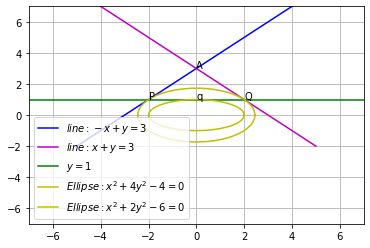
\includegraphics[scale=0.5]{c1.jpg}
    \caption{Tangents at $\vec{q_1}$}
    \label{fig:Bisector}
\end{figure}

\begin{table}[h]
	\centering
\setlength\extrarowheight{2pt}
	\begin{tabular}{|c|c|c|}
		\hline
		\textbf{Symbol} & \textbf{Value} & \textbf{Description} \\
		\hline
		$\vec{A}$ & (0,3) & point $\vec{A}$\\
		\hline
		$\vec{P}$ & (-2,1) & point $\vec{P}$\\
		\hline
		$\vec{Q}$ & (2,1) & point $\vec{Q}$\\
		\hline
		$\vec{q_1}$ & (0,1) & point $\vec{q_1}$\\
		\hline
	\end{tabular}
\end{table}


\begin{figure}[H]
    \centering
    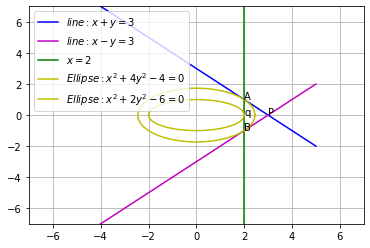
\includegraphics[scale=0.5]{c2.jpg}
    \caption{Tangents at $\vec{q_2}$}
    \label{fig:Bisector}
\end{figure}

\begin{table}[h]
	\centering
\setlength\extrarowheight{2pt}
	\begin{tabular}{|c|c|c|}
		\hline
		\textbf{Symbol} & \textbf{Value} & \textbf{Description} \\
		\hline
		$\vec{A}$ & (2,1) & point $\vec{A}$\\
		\hline
		$\vec{B}$ & (2,-1) & point $\vec{B}$\\
		\hline
		$\vec{P}$ & (3,0) & point $\vec{P}$\\
		\hline
		$\vec{q_2}$ & (2,0) & point $\vec{q_2}$\\
		\hline
	\end{tabular}
\end{table}

    The above constructions are realized by executing the following codes.
    
\begin{table}[H]
\begin{tabular}{|l|c|c|c|c|c|c|c|c}\hline\textbf{https://github.com/BavyaVemulapalli}\\
    \textbf{/FWC-IITH/tree/main/Conic/Codes} \\ \hline
\end{tabular}
\end{table}

\section{Conclusion}

    \begin{flushleft}
        Hence we proved that the tangents at $\vec{A}$ and $\vec{B}$ of the ellipse $\vec{x^\top}\myvec{1 & 0 \\ 0 & 2}\vec{x} - 6 = 0$ are at right angle.
    \end{flushleft}

\end{document}